\documentclass[aspectratio=169,xcolor=dvipsnames]{beamer}

\usetheme{TJU}
\usepackage{svg}
\usepackage{booktabs} % \toprule \midrule \bottomrule
\usepackage{graphics}
\usepackage{tikz}
\usepackage{listings}

%----------------------------------------------------------------------------------------
%	TITLE PAGE
%----------------------------------------------------------------------------------------
\title[Short]{TJU Beamer Template}
\subtitle[Short]{Subtitle}
\author[Zeng]{jianhao zeng}
\institute{School of Electrical and Information Engineering \\ Tianjin University}
\date[2023]{\today}

%----------------------------------------------------------------------------------------
%	PRESENTATION SLIDES
%----------------------------------------------------------------------------------------
\begin{document}

    \begin{frame}
        \titlepage
    \end{frame}

    \begin{frame}{Overview}
        \tableofcontents
    \end{frame}

%------------------------------------------------
\section{First Section}
%------------------------------------------------
\begin{frame}{Bullet Points}
    \begin{itemize}
        \item Lorem ipsum dolor sit amet, consectetur adipiscing elit
        \item Aliquam blandit faucibus nisi, sit amet dapibus enim tempus eu
        \item Nulla commodo, erat quis gravida posuere, elit lacus lobortis est, quis porttitor odio mauris at libero
        \item Nam cursus est eget velit posuere pellentesque
        \item Vestibulum faucibus velit a augue condimentum quis convallis nulla gravida
    \end{itemize}
\end{frame}

%------------------------------------------------
\section{Second Section}
%------------------------------------------------
\begin{frame}{Blocks of Highlighted Text}
    In this slide, some important text will be \alert{highlighted} because it's important. Please, don't abuse it.

    \begin{block}{Block}
        Sample text
    \end{block}

    \begin{alertblock}{Alertblock}
        Sample text in red box
    \end{alertblock}

    \begin{examples}
        Sample text in green box. The title of the block is ``Examples".
    \end{examples}
\end{frame}


%------------------------------------------------
\section{Third Section}
%------------------------------------------------
\begin{frame}{Multiple Columns}
    \begin{columns}[c]
        \column{.45\textwidth}
        \textbf{Heading}
        \begin{enumerate}
            \item Statement
            \item Explanation
            \item Example
        \end{enumerate}

        \column{.5\textwidth}
        Lorem ipsum dolor sit amet, consectetur adipiscing elit. Integer lectus nisl, ultricies in feugiat rutrum, porttitor sit amet augue. Aliquam ut tortor mauris. Sed volutpat ante purus, quis accumsan dolor.
    \end{columns}
\end{frame}


%------------------------------------------------
\section{Fourth Section}
%------------------------------------------------
\begin{frame}{Table}
    \begin{table}
        \begin{tabular}{l l l}
            \toprule
            \textbf{Treatments} & \textbf{Response 1} & \textbf{Response 2} \\
            \midrule
            Treatment 1         & 0.0003262           & 0.562               \\
            Treatment 2         & 0.0015681           & 0.910               \\
            Treatment 3         & 0.0009271           & 0.296               \\
            \bottomrule
        \end{tabular}
        \caption{Table caption}
    \end{table}
\end{frame}

%------------------------------------------------
\section{Fifth Section}
%------------------------------------------------
\begin{frame}{Theorem}
    \begin{theorem}[Mass--energy equivalence]
        $E = mc^2$
    \end{theorem}
    \begin{equation}
        c^{2} = a^{2} + b^{2}
    \end{equation}
\end{frame}

%------------------------------------------------
\section{Sixth Section}
%------------------------------------------------
\begin{frame}{Figure}
    \begin{figure}
        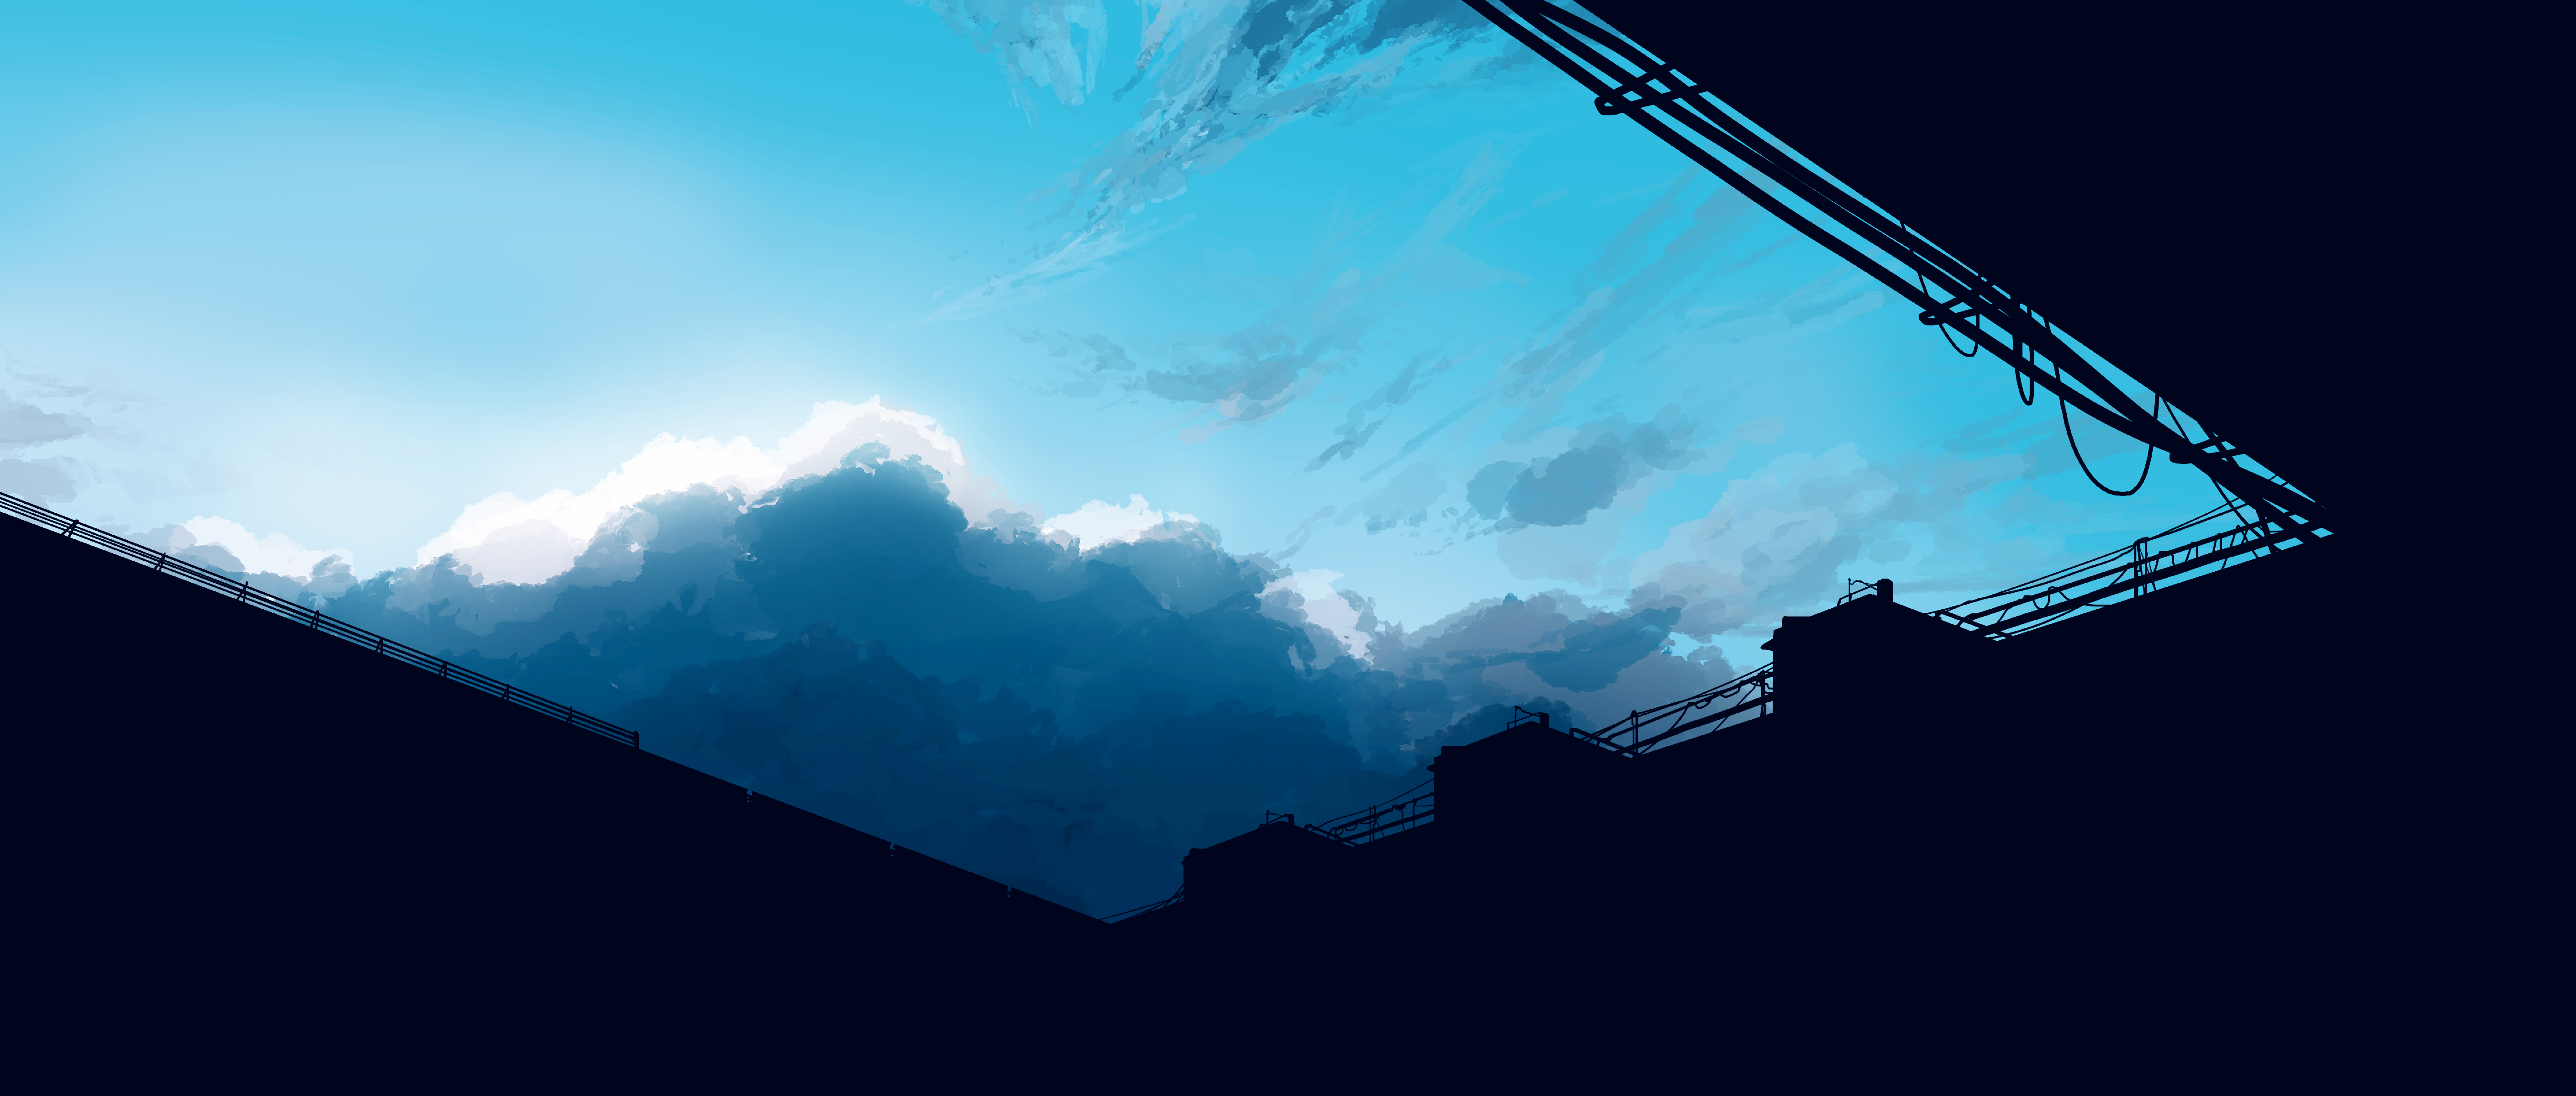
\includegraphics[width=0.8\linewidth]{background.jpg}
    \end{figure}
\end{frame}


%------------------------------------------------
\section{End}
%------------------------------------------------
\begin{frame}
    \Huge{\centerline{\textbf{The End}}}
\end{frame}


\end{document}
